\chapter{Fondamenti teorici}

Prima di addentrarsi nei dettagli implementativi dell'architettura realizzata, è necessario costruire un solido quadro teorico che permetta di comprendere le scelte progettuali con piena consapevolezza del loro significato. Questo capitolo tratta i modelli formali di sicurezza, i principi di progettazione sicura, le tecnologie crittografiche alla base delle comunicazioni protette e gli strumenti specifici impiegati nel progetto.

\section{Il modello Zero Trust}

Il termine Zero Trust fu coniato da John Kindervag nel 2010, durante il suo lavoro presso Forrester Research; le radici concettuali del modello affondano tuttavia in una critica più antica al modello perimetrale. L'idea tradizionale di sicurezza informatica era quella del castello con il fossato: una rete interna considerata sicura, protetta da un perimetro difensivo verso l'esterno. Tutto ciò che si trovava all'interno del perimetro godeva di un livello implicito di fiducia. Questa assunzione si è rivelata pericolosa: una volta violato il perimetro, un attaccante poteva muoversi lateralmente attraverso la rete con scarsa resistenza.

Il modello Zero Trust rovescia questa logica in modo radicale. Nessuna entità, né utente, né dispositivo, né servizio, è considerata affidabile per default, indipendentemente dalla sua posizione nella rete. Ogni accesso deve essere esplicitamente autenticato, autorizzato e continuamente validato. La rete stessa smette di essere un elemento di fiducia e diventa semplicemente un mezzo di trasporto.

Il riferimento normativo più autorevole per l'implementazione pratica del modello è la pubblicazione NIST SP 800-207, \textit{Zero Trust Architecture}, pubblicata nel 2020. Questo documento definisce i principi fondamentali del modello e identifica i componenti logici di un'architettura Zero Trust.

\subsection{Principi fondamentali secondo NIST 800-207}

La pubblicazione NIST SP 800-207 articola il modello Zero Trust attorno a 7 principi fondamentali:

\begin{itemize}
\item tutte le risorse sono considerate non affidabili, indipendentemente dalla loro posizione nella rete;
\item tutte le comunicazioni devono essere protette, anche quelle interne alla rete aziendale;
\item l'accesso alle risorse deve essere concesso su base per-sessione e con il minimo privilegio necessario;
\item l'accesso è determinato da policy dinamiche che tengono conto dell'identità, del dispositivo, della rete e di altri attributi contestuali;
\item l'integrità e la sicurezza di tutti i dispositivi connessi devono essere monitorate e verificate;
\item l'autenticazione e l'autorizzazione devono essere eseguite in modo dinamico e rigoroso prima di consentire l'accesso;
\item l'organizzazione deve raccogliere quante più informazioni possibile sullo stato delle risorse e delle comunicazioni, e usarle per migliorare continuamente la postura di sicurezza.
\end{itemize}

\subsection{Policy Enforcement Point e Policy Decision Point}

L'architettura Zero Trust secondo NIST si articola attorno a 2 componenti logici principali. Il Policy Enforcement Point (PEP) è il punto in cui il traffico viene intercettato e le decisioni di accesso vengono applicate. Il PEP non decide autonomamente: riceve un verdetto da un'entità separata e lo esegue, consentendo o bloccando la richiesta. Il Policy Decision Point (PDP) è invece il componente che valuta le policy e produce il verdetto. Nel modello NIST, il PDP si compone a sua volta di un Policy Engine, che applica le regole di accesso, e di un Policy Administrator, che traduce il verdetto in istruzioni operative per il PEP.

La separazione tra PEP e PDP è un requisito architetturale fondamentale, non una mera convenzione. Essa garantisce che la logica di applicazione delle regole e la logica di definizione delle regole siano mantenute distinte, riducendo la complessità di ciascun componente e limitando il raggio di impatto di una potenziale compromissione.

Nel progetto descritto in questo elaborato, il PEP è implementato da Envoy Proxy, mentre il PDP è realizzato dalla combinazione del Security Orchestrator, del modello di AI e dal motore di policy OPA.

\section{Modelli formali di controllo degli accessi}
\label{sec:Modelli formali di controllo degli accessi}

La teoria del controllo degli accessi ha radici che risalgono agli anni Settanta e ha prodotto modelli formali che ancora oggi informano la progettazione dei sistemi di sicurezza moderni. Comprendere questi modelli è essenziale per valutare le scelte architetturali di qualsiasi sistema che gestisca risorse con livelli di sensibilità differenziati.

\subsection{Controllo degli accessi basato su ruoli}

Il Role-Based Access Control (RBAC), standardizzato nella pubblicazione ANSI/INCITS 359-2004, è un modello di controllo degli accessi in cui i permessi non sono assegnati direttamente agli utenti ma ai ruoli, e gli utenti acquisiscono i permessi in virtù dell'appartenenza a uno o più ruoli. Il riferimento NIST specifico per RBAC è invece la pubblicazione NIST IR 7316, che definisce le specifiche funzionali del modello senza costituire essa stessa lo standard ANSI/INCITS. Questo approccio semplifica notevolmente la gestione degli accessi in sistemi con molti utenti e molte risorse.

Nel progetto il modello Role-Based Access Control costituisce il livello di base per l'astrazione e la gestione delle identità all'interno del sistema di autorizzazione. A differenza delle implementazioni RBAC tradizionali, dove il ruolo determina staticamente i permessi di accesso a specifiche risorse, in questa architettura il ruolo funge da livello di disaccoppiamento organizzativo.
Le identità degli utenti vengono veicolate tramite token JWT dai quali viene estratto un attributo di business (ad esempio: \texttt{guest}, \texttt{operator}, \texttt{manager}, \texttt{admin}). Il motore di policy utilizza una mappa associativa per convertire questi ruoli organizzativi in etichette di sicurezza. 

Invece di assegnare individualmente complessi set di parametri ad ogni singolo dipendente, l'appartenenza a un ruolo popola dinamicamente gli attributi strutturali necessari ai modelli successivi.

\subsection{Controllo degli accessi basato su attributi}

Il modello Attribute-Based Access Control (ABAC) estende RBAC introducendo la valutazione di attributi arbitrari relativi al soggetto, alla risorsa, all'ambiente e all'azione richiesta. Le decisioni di accesso non dipendono solo dal ruolo dell'utente, ma da una combinazione di attributi che può includere l'ora della richiesta, il tipo di dispositivo, il livello di rischio corrente e qualsiasi altra informazione contestuale rilevante.

Nell'implementazione realizzata, l'approccio ABAC permette di superare i limiti di un'autorizzazione puramente statica valutando il contesto di ogni singola richiesta in tempo reale. Agli attributi dell'oggetto (come il percorso specifico dell'endpoint e il metodo HTTP) vengono associati metadati quantitativi intrinseci di rischio. 

L'elemento architetturale chiave introdotto in questa fase è la valutazione degli attributi ambientali, rappresentati specificamente da uno \textit{score di rischio} continuo. Attraverso questo scambio di attributi, l'ABAC realizza concretamente il principio della valutazione continua del rischio.

\subsection{Il modello Bell-LaPadula}

Il modello Bell-LaPadula, proposto da David Elliott Bell e Leonard J. LaPadula nel 1973 per conto della United States Air Force, è il modello formale di riferimento per la confidenzialità delle informazioni. Il suo obiettivo è impedire che informazioni riservate fluiscano verso soggetti non autorizzati a riceverle.

Il modello introduce il concetto di livello di sicurezza, originariamente costituito da 2 dimensioni che formano una struttura a reticolo: una gerarchia totalmente ordinata e un insieme non gerarchico di compartimenti o categorie. Nel progetto realizzato, i livelli gerarchici adottati sono 5: PUBLIC, INTERNAL, CONFIDENTIAL, SECRET e TOP\_SECRET, in ordine crescente di sensibilità. A questi si affiancano specifiche categorie (es. \textit{nuclear, security}). Un accesso è consentito solo se, oltre a soddisfare i vincoli di livello, il soggetto possiede un insieme di categorie che include (superset) tutte quelle richieste dall'oggetto.

Il modello formale completo si fonda su 3 proprietà fondamentali del Mandatory Access Control (MAC). La \textit{Simple Security Property} (o proprietà \textit{no read-up}) stabilisce che un soggetto può leggere un oggetto solo se il suo livello di autorizzazione domina quello dell'oggetto. La \textit{Star Property} (o proprietà \textit{no write-down}) stabilisce che un soggetto non può scrivere su un oggetto con livello di classificazione inferiore al proprio, impedendo il declassamento illecito delle informazioni. La terza proprietà, la \textit{Discretionary Security Property} (ds-property), regola gli accessi discrezionali tramite una matrice degli accessi sovrapposta al controllo obbligatorio basato sui livelli: un soggetto può accedere a un oggetto solo se, oltre a soddisfare le 2 proprietà precedenti, la matrice degli accessi discrezionali autorizza esplicitamente quella particolare combinazione di soggetto, oggetto e modalità di accesso. Il progetto implementa le prime 2 proprietà; la ds-property non è oggetto di un'implementazione dedicata, costituendo una lacuna teorica rispetto alla formulazione completa del modello.

\subsubsection{Esempio di sanificazione}
Tuttavia, l'implementazione in OPA estende questo concetto introducendo la figura del \textit{Trusted Subject}: viene definita una deroga controllata alla \textit{Star Property} per consentire a un utente \texttt{admin} (TOP\_SECRET) di scrivere su una specifica rotta sanitizzata di livello inferiore (SECRET), permettendo così una de-classificazione sicura delle informazioni.

\begin{figure}[h]
    \centering
    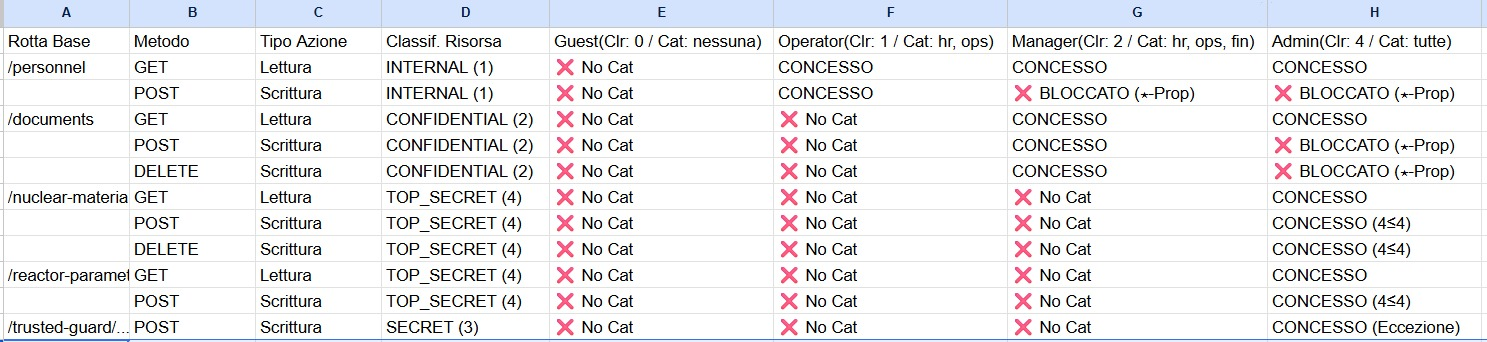
\includegraphics[width=0.9\textwidth]{immagini/bell-lapadula.jpeg}
    \caption{Tabella Bell\-Lapadula}
    \label{fig:BellLapadula}
\end{figure}

\subsection{Algoritmo di fiducia}

L'algoritmo di fiducia implementato nel file \texttt{policy.rego} di OPA si distingue per la sua architettura \textit{ibrida}, che fonde metodologie di controllo rigido degli attributi (tipiche dei sistemi Mandatory Access Control) con meccanismi di controllo basato sul punteggio.

\subsubsection{Controllo degli Attributi: Modello Bell-LaPadula}
La componente deterministica dell'algoritmo si basa su un'implementazione del modello di confidenzialità Bell-LaPadula (BLP).
\subsubsection{Controllo basato sul punteggio: valutazione dinamica del rischio}
A valle del controllo deterministico, l'algoritmo ibrido introduce una fase di computazione algoritmica basata sulla somma e sottrazione di attributi di rischio continuo. Questo garantisce che credenziali compromesse (ma formalmente valide nel modello BLP) non siano sufficienti per finalizzare un attacco.

Per ogni singola richiesta HTTP, l'algoritmo valuta:
\begin{itemize}
    \item \textit{beneficio dell'operazione} ($B$): un indice quantitativo pre-assegnato al metodo e alla rotta (es. $0.9$ per rotte critiche, $0.6$ per risorse interne);
    \item \textit{punteggio AI di minaccia} ($A$): un attributo dinamico valutato in tempo reale che quantifica il livello di rischio della richiesta.
    \item \textit{beneficio netto}: \begin{equation}
    B_{netto} =  B - A \end{equation}
    \item \textit{soglia di beneficio netto minimo} ($B_{m}$): il livello minimo di beneficio netto richiesto per la specifica transazione(es. $0.8$ per rotte critiche, $0.3$ per risorse interne);
\end{itemize}

Il blocco di autorizzazione finale si risolve tramite la disuguaglianza algebrica :
\begin{equation}
    B - A \geq B_{m}
\end{equation}
Questa disuguaglianza impone che un'operazione venga completata unicamente se il suo vantaggio contestuale eccede la soglia di beneficio netto minimo richiesto configurato per lo specifico endpoint. È importante chiarire la semantica di $B$ per evitare un'interpretazione fuorviante: il parametro non misura la sensibilità o criticità della risorsa, ma il beneficio operativo, cioè quanto è necessario che l'operazione vada a buon fine per il corretto funzionamento del sistema (ad esempio, un'operazione di lettura su una rotta di monitoraggio essenziale per la sicurezza dell'impianto può avere beneficio più alto di una scrittura su una risorsa interna non urgente, indipendentemente dalla classificazione di sensibilità del dato). Il parametro che effettivamente codifica la criticità della risorsa è $B_{m}$: alle rotte più sensibili viene assegnata una soglia di beneficio netto minimo accettato molto più alta, cosicché anche un beneficio numerico elevato non comprometta la sicurezza complessiva, poiché la disuguaglianza richiede comunque che il punteggio di rischio AI resti contenuto entro un margine ristretto. I due parametri sono quindi calibrati congiuntamente per ciascuna rotta, e non in modo indipendente: un beneficio alto su una rotta critica è sempre accompagnato da una soglia di beneficio netto minimo accettato proporzionalmente più severa.


\section{Principi di progettazione sicura}

Parallelamente ai modelli formali, la letteratura di sicurezza informatica ha elaborato un insieme di principi di progettazione che guidano la costruzione di sistemi resistenti. Questi principi, enunciati originariamente da Jerome Saltzer e Michael Schroeder nel loro articolo seminale del 1975 \textit{The Protection of Information in Computer Systems}, rimangono di piena attualità e informano ogni scelta architetturale significativa.

\subsection{Economy of mechanism}

Il principio di economy of mechanism afferma che i meccanismi di sicurezza devono essere progettati per essere il più semplici e piccoli possibile. La semplicità riduce la probabilità di errori implementativi, semplifica la verifica della correttezza e limita la superficie di attacco. Un meccanismo complesso è più difficile da capire, da testare e da mantenere nel tempo.

Nel progetto, questo principio si manifesta nella scelta di componenti con responsabilità ben definite e limitate. nftables si occupa esclusivamente del filtraggio del traffico a livello di rete, Envoy gestisce la terminazione TLS e la delega dell'autorizzazione, OPA valuta le policy in linguaggio Rego: ciascuno di questi componenti rispetta pienamente il principio.

\subsection{Fail-safe defaults}

Il principio di fail-safe defaults stabilisce che, in assenza di una decisione di autorizzazione esplicita, il sistema deve negare l'accesso. Il comportamento predefinito deve essere il rifiuto, non il consenso. Un sistema che fallisce in modo sicuro limita i danni derivanti da errori di configurazione o da condizioni impreviste.

Questo principio è visibile in più punti dell'architettura. La policy OPA definisce \texttt{default allow = false}, garantendo che qualsiasi richiesta per cui non sia applicabile una regola esplicita di consenso venga negata automaticamente. Analogamente, la catena di nftables configura la policy di default del chain \texttt{input} a DROP, in modo che solo il traffico esplicitamente consentito possa raggiungere il sistema.

\subsection{Complete mediation}

Il principio di complete mediation afferma che ogni accesso a ogni risorsa deve essere verificato, senza eccezioni e senza possibilità di aggirare il meccanismo di controllo. Non deve esistere alcun percorso che consenta di accedere a una risorsa senza passare attraverso il punto di autorizzazione.

L'architettura del progetto garantisce la complete mediation attraverso la topologia di rete. Il Business DB, che contiene i dati più sensibili dell'applicazione, è raggiungibile esclusivamente dal servizio Business Logic attraverso la rete isolata Back-Net. Ogni richiesta al servizio applicativo deve necessariamente transitare per Envoy, che intercetta il traffico e delega l'autorizzazione prima di instradare la richiesta. Come descritto nel Capitolo 3, non esiste alcun percorso diretto dall'esterno, dal Security Orchestrator o dal motore PDP verso il Business DB: nessuno dei componenti del piano decisionale dispone di credenziali proprie su tale database, e l'unico punto di accesso resta il servizio Business Logic attraverso la rete isolata Back-Net.

\subsection{Separation of privilege}

Il principio di separation of privilege afferma che un sistema non dovrebbe concedere l'accesso o eseguire un'operazione sulla base di un'unica condizione, ma richiedere la soddisfazione di più condizioni indipendenti. La separazione dei privilegi riduce il rischio che la compromissione di un singolo fattore sia sufficiente a violare la sicurezza del sistema.

Nel progetto, la decisione di accesso richiede la soddisfazione simultanea di più condizioni: l'utente deve avere un livello di clearance adeguato alla classificazione della risorsa, un trust score superiore alla soglia minima richiesta dalla zona, l'enrollment MFA dove richiesto, un dispositivo di tipo consentito e una provenienza di rete autorizzata. La compromissione di un solo fattore, ad esempio il furto di credenziali, non è sufficiente a ottenere l'accesso se il dispositivo utilizzato non corrisponde all'impronta JA3 attesa o se il trust score è al di sotto della soglia.

\subsection{Least privilege}

Il principio del minimo privilegio afferma che ogni entità del sistema, utente, processo o componente, deve operare con il minimo insieme di permessi necessario per svolgere le proprie funzioni. Questo limita i danni in caso di compromissione e riduce la superficie di attacco disponibile.

L'applicazione di questo principio è pervasiva nell'architettura. Il servizio Business Logic non si connette al database con un'unica utenza a privilegi globali, ma utilizza 3 credenziali MongoDB distinte e role-scoped (\texttt{operator\_client}, \texttt{manager\_client}, \texttt{admin\_client}), ciascuna abilitata alle sole collection pertinenti al rispettivo livello. In questo modo il principio del minimo privilegio è applicato non solo dalla policy di autorizzazione, ma anche dalle credenziali con cui si raggiunge effettivamente il dato, fornendo un secondo strato di difesa indipendente. Ogni microservizio, analogamente, opera all'interno del segmento di rete strettamente necessario alle proprie funzioni.

\subsection{Open design}

Il principio di open design afferma che la sicurezza di un sistema non deve dipendere dalla segretezza del suo meccanismo di protezione, ma esclusivamente dalla segretezza delle chiavi o delle credenziali. Un sistema la cui sicurezza dipende dall'oscurità della propria implementazione risulta strutturalmente debole: qualora il meccanismo venga scoperto, l'efficacia della protezione viene del tutto compromessa.

Nel progetto, i meccanismi di protezione sono basati su standard aperti e ampiamente verificati: TLS 1.3 per la cifratura delle comunicazioni, X.509 per i certificati, SHA-256 per gli hash di integrità. La sicurezza risiede nella segretezza delle chiavi private, non nella segretezza degli algoritmi. Le policy OPA sono espresse in Rego, un linguaggio leggibile e auditabile, la cui correttezza può essere verificata in modo indipendente; il documento non include tuttavia il codice Rego della policy né nel corpo del testo né in appendice, il che rende di fatto impossibile per il lettore verificare l'affermazione di auditabilità sulla base del materiale presentato.

\subsection{Psychological acceptability}

Il principio di psychological acceptability afferma che i meccanismi di sicurezza devono essere progettati in modo da non creare ostacoli eccessivi agli utenti legittimi. Se i controlli di sicurezza sono troppo onerosi, gli utenti troveranno modi per aggirarli. La sicurezza deve essere praticabile, non solo teoricamente corretta.

In un'architettura Zero Trust, questo principio si traduce nella trasparenza dei controlli: l'autenticazione e l'autorizzazione avvengono in modo il più possibile automatico, senza richiedere azioni aggiuntive all'utente se non nei casi in cui il rischio lo giustifichi. Nell'implementazione realizzata, tuttavia, l'autenticazione a più fattori è richiesta a ogni singolo login, indipendentemente dal livello di rischio della sessione: dopo la verifica di username e password, il sistema emette sempre un codice OTP monouso inviato via email che l'utente deve confermare prima che venga rilasciato il token di sessione. Questa scelta è in tensione diretta con il principio appena enunciato, che prevede l'introduzione di attriti aggiuntivi solo quando il rischio lo giustifica e non in modo incondizionato; va inoltre osservato che l'OTP via email è generalmente considerato in letteratura un secondo fattore relativamente debole, una caratteristica rilevante per un sistema che protegge un impianto nucleare.

\section{Crittografia applicata e TLS}

Le comunicazioni sicure all'interno dell'architettura si fondano su protocolli crittografici standard. La comprensione dei meccanismi sottostanti è necessaria per valutare le garanzie di sicurezza offerte dal sistema.

\subsection{Transport Layer Security}

Il protocollo TLS (Transport Layer Security) è lo standard de facto per la protezione delle comunicazioni su reti non affidabili. La versione corrente, TLS 1.3, definita nella RFC 8446, introduce significativi miglioramenti rispetto alle versioni precedenti: eliminazione di suite crittografiche deboli, riduzione della latenza dell'handshake da 2 round-trip a uno, e forward secrecy obbligatoria attraverso l'uso esclusivo di scambi di chiave effimeri basati su Diffie-Hellman.

Il processo di handshake TLS stabilisce un canale sicuro tra client e server attraverso una sequenza di messaggi che negozia le suite crittografiche, autentica le parti e deriva le chiavi di sessione. Il risultato è un canale che garantisce confidenzialità (attraverso la cifratura simmetrica), integrità (attraverso MAC o AEAD) e autenticazione (attraverso certificati digitali). È opportuno precisare che la forward secrecy obbligatoria di TLS 1.3 riguarda esclusivamente le chiavi di sessione, derivate in modo effimero a ogni handshake: i certificati client statici impiegati nel mutual TLS non beneficiano direttamente di questa proprietà, poiché la chiave privata associata al certificato resta fissa nel tempo. La compromissione di tale chiave privata, pur non esponendo le sessioni passate già concluse, comprometterebbe comunque l'autenticazione futura del client fino alla revoca o al rinnovo del certificato.

Nel progetto, Envoy termina le connessioni TLS in ingresso, gestendo il processo di handshake e l'estrazione dei metadati crittografici attraverso il TLS Inspector. L'uso di TLS 1.3 è rilevante anche per il JA3 fingerprinting: client che negoziano con cipher suite o versioni TLS datate producono hash JA3 distinti e riconoscibili, consentendo al sistema di identificare connessioni anomale anche in presenza di credenziali valide.

\subsection{Mutual TLS}

Il mutual TLS (mTLS) è un'estensione del protocollo TLS in cui entrambe le parti, client e server, si autenticano reciprocamente mediante certificati digitali X.509. Nel TLS standard, solo il server presenta un certificato per autenticarsi al client; nell'mTLS, anche il client è tenuto a presentare un certificato valido, firmato da una Certificate Authority (CA) fidata dal server.

Questo meccanismo è particolarmente adatto agli ambienti Zero Trust, perché fornisce un'autenticazione forte basata su crittografia a chiave pubblica, indipendente da credenziali riutilizzabili come username e password. Un client che non disponga di un certificato valido firmato dalla CA interna non può stabilire una connessione, indipendentemente da qualsiasi altra credenziale. Va segnalato che il progetto non prevede alcun meccanismo di revoca dei certificati, né tramite Certificate Revocation List (CRL) né tramite Online Certificate Status Protocol (OCSP): in un'architettura Zero Trust la capacità di revocare rapidamente un certificato compromesso costituisce un requisito fondamentale, che in questo caso resta privo di copertura. Una mitigazione parziale, non implementata nella versione corrente del progetto ma proponibile come lavoro futuro, consisterebbe nell'adozione di certificati a vita molto breve (short-lived certificates, tipicamente con validità di ore) rilasciati da una CA interna automatizzata: questo approccio, diffuso in architetture Zero Trust moderne, riduce drasticamente la finestra di esposizione di un certificato compromesso senza richiedere l'infrastruttura aggiuntiva di un servizio CRL o OCSP, spostando di fatto il problema della revoca verso quello, più gestibile, del rinnovo automatico frequente.

Nel progetto, Envoy è configurato con \texttt{require\_client\_certificate: false}, rendendo facoltativa la presentazione di un certificato client firmato dalla CA interna. I certificati sono generati tramite OpenSSL con il parametro di estensione \texttt{extendedKeyUsage=client Auth}, garantendo che possano essere utilizzati esclusivamente per l'autenticazione del client. Al termine dell'handshake, quando un certificato è presente, Envoy ne inietta i metadati nell'header \texttt{X-Forwarded-Client-Cert}; il Security Orchestrator li interpreta per risolvere l'identità del soggetto richiedente in modo crittograficamente verificato e li inoltra al livello di policy. Questa configurazione è in tensione con la filosofia Zero Trust dichiarata per il progetto: rendere facoltativo il certificato a livello TLS significa demandare per intero la verifica al Security Orchestrator e, più a valle, al servizio Identity (si veda la discussione al Capitolo 3 e alla Sezione~\ref{sec:autenticazionestandard}), introducendo un punto di fiducia implicita su Envoy. Sebbene il controllo applicativo successivo blocchi correttamente le richieste prive di certificato per i ruoli che lo richiedono, l'assenza di enforcement a livello di trasporto resta una scelta architetturale che meriterebbe un'analisi critica più esplicita nel documento, dato che espone comunque superficie applicativa a un client non ancora autenticato a livello TLS.

\subsection{JA3 fingerprinting}

Il JA3 fingerprinting è una tecnica di identificazione del client basata sui parametri dell'handshake TLS. Sviluppata da John Althouse, Jeff Atkinson e Josh Atkins presso Salesforce nel 2017, costruisce una firma identificativa del client a partire da 5 campi dell'handshake: la versione TLS proposta, le cipher suite supportate, le estensioni TLS incluse, i gruppi di curve ellittiche e i formati di punto ellittico.

Questi 5 campi vengono concatenati in una stringa con separatori definiti e poi sottoposti a hashing MD5, producendo un identificatore di 32 caratteri esadecimali che è caratteristico della combinazione di libreria TLS e configurazione utilizzata dal client. Client diversi, anche se usano le stesse credenziali, produrranno hash JA3 differenti se il loro stack TLS è diverso. Questo rende il JA3 uno strumento utile per rilevare impersonificazioni, bot e client anomali anche quando le credenziali presentate sono valide. La tecnica presenta tuttavia limiti ben noti che il progetto non affronta esplicitamente: un tasso di collisione non trascurabile tra client diversi che condividono la stessa libreria e versione TLS, la possibilità di spoofing intenzionale dell'impronta da parte di un attaccante che ne conosca i parametri di calcolo, e una progressiva perdita di efficacia con l'adozione di TLS 1.3, dove la riduzione della variabilità osservabile dell'handshake limita la distintività delle impronte, fino all'inutilizzabilità completa quando il client adotta l'estensione Encrypted Client Hello (ECH), che cifra interamente i parametri dell'handshake altrimenti usati per il calcolo del fingerprint.

Nel progetto, Envoy è configurato con \texttt{enable\_ja3\_fingerprinting: true} nel filtro TLS Inspector. Envoy espone la stringa JA3 grezza come variabile di metadato e la inietta negli header della richiesta inoltrata al Security Orchestrator. È quest'ultimo a calcolarne il digest MD5, ottenendo l'hash a 32 caratteri esadecimali.

\section{Componenti tecnologici}

\subsection{nftables}

nftables è il framework di filtraggio dei pacchetti del kernel Linux, introdotto come successore di iptables a partire dal kernel 3.13. A differenza di iptables, nftables offre una sintassi unificata per IPv4 e IPv6, supporto nativo per set e mappe di indirizzi, e un'architettura interna più efficiente basata su una macchina virtuale integrata nel kernel.

Nel progetto, nftables opera come firewall di rete posizionato tra il client esterno e il
  resto dell'infrastruttura. La sua configurazione definisce una tabella \texttt{inet filter} le
  cui 3 catene principali, \texttt{input}, \texttt{forward} e \texttt{output}, adottano tutte
  una policy di default DROP, così che solo il traffico esplicitamente consentito venga
  accettato in ciascuna direzione. In particolare la catena \texttt{output} ammette il solo
  traffico in uscita strettamente necessario, ossia la risoluzione DNS e la comunicazione verso
  i microservizi interni. La catena \texttt{input} accetta il traffico locale, il traffico
  appartenente a connessioni già stabilite e il traffico TCP verso la porta di Envoy da
  indirizzi non presenti nella lista di blocco, loggando ogni pacchetto accettato o rifiutato
  tramite il gruppo NFLOG 100.

\subsection{Snort}

Snort è un sistema di rilevamento e prevenzione delle intrusioni di rete (NIDS/NIPS) open source, originariamente sviluppato da Marty Roesch nel 1998 e successivamente acquisito da Cisco. Opera analizzando il traffico di rete in tempo reale, confrontando i pacchetti catturati con un insieme di regole configurabili per rilevare pattern corrispondenti ad attività malevole note.

Snort può operare in 3 modalità: sniffer (stampa i pacchetti sulla console), packet logger (salva i pacchetti su disco) e network intrusion detection system (analizza i pacchetti e genera alert). Nel progetto, Snort è configurato in modalità NIDS con output su console, condivide lo stack di rete del container firewall tramite la direttiva \texttt{network\_mode: service:firewall}, e monitora l'interfaccia eth0.

La regola custom configurata utilizza il preprocessore \texttt{sfportscan} per rilevare scansioni di porte, abilitato con il parametro \texttt{sense\_level: low} per minimizzare i falsi positivi. Una regola Snort aggiuntiva segnala esplicitamente la rilevazione di un port scan TCP quando vengono rilevati più di 5 pacchetti SYN dalla stessa sorgente nell'arco di 5 secondi. Questo scenario è uno dei vettori di attacco testati esplicitamente nel progetto, con client di test che simulano la scansione rapida di un intervallo di porte.

\subsection{Envoy Proxy}

Envoy è un proxy L4/L7 open source sviluppato originariamente da Lyft e successivamente donato alla Cloud Native Computing Foundation (CNCF). È progettato per essere il piano dati di architetture a microservizi, gestendo la comunicazione tra servizi con funzionalità avanzate di load balancing, circuit breaking, osservabilità e sicurezza.

Nel contesto del progetto, Envoy svolge il ruolo di Policy Enforcement Point. La sua configurazione YAML definisce un listener sulla porta 8443 che, grazie al filtro \texttt{tls\_inspector}, ispeziona i parametri dell'handshake TLS prima ancora che la connessione sia completamente stabilita. Il filtro \texttt{http\_connection\_manager} gestisce la connessione HTTP una volta che l'handshake TLS è concluso. Envoy è configurato per richiedere il certificato client e per loggare in formato JSON strutturato una serie di informazioni sulla connessione, tra cui la versione TLS, la cipher suite, l'indirizzo remoto e l'hash JA3, propagando l'header \texttt{X-Request-ID} per garantire la tracciabilità.

Il protocollo \texttt{ext\_authz} di Envoy permette di delegare la decisione di autorizzazione a un servizio esterno, in questo caso il Security Orchestrator, prima di instradare la richiesta verso il backend. Questo è il meccanismo attraverso cui si realizza la separazione tra PEP e PDP.

\subsection{Open Policy Agent e Rego}

Open Policy Agent (OPA) è un motore di policy general-purpose open source, mantenuto dalla CNCF, che permette di esprimere e valutare policy in modo unificato attraverso diversi domini applicativi. OPA riceve in input un documento JSON che rappresenta il contesto della richiesta e valuta le policy scritte in Rego, restituendo un documento JSON che rappresenta la decisione.

Rego è un linguaggio dichiarativo derivato da Datalog, progettato specificamente per la definizione di policy. A differenza di un linguaggio imperativo, in Rego si descrive \textit{cosa} deve essere vero perché una policy sia soddisfatta, non \textit{come} verificarlo. Questo rende le policy leggibili, componibili e verificabili in modo indipendente rispetto al codice applicativo che le esegue.

Nel progetto, OPA opera come Policy Decision Point puro. Riceve dall'Orchestratore un payload che contiene ruolo dell'utente, risorsa richiesta, metodo e score del rischio generato dal modello di AI. OPA valuta tutte queste condizioni, come descritto in precedenza nella \autoref{sec:Modelli formali di controllo degli accessi}, restituendo un verdetto binario allow/deny. La separazione tra la policy e il codice che la applica garantisce che le regole possano essere modificate, testate e verificate in modo indipendente dalla logica applicativa.

\subsection{Splunk}

Splunk è una piattaforma di analisi operativa dei dati macchina, ampiamente utilizzata come SIEM (Security Information and Event Management) in ambito enterprise. Raccoglie log da sorgenti eterogenee, li normalizza, li indicizza e li rende ricercabili e correlabili attraverso il linguaggio di query SPL (Search Processing Language).

Nel progetto, Splunk opera come centro di osservabilità dell'intera architettura. Ogni microservizio invia i propri log a Splunk tramite l'HTTP Event Collector (HEC), un endpoint HTTP che accetta eventi in formato JSON autenticati tramite token. L'uso del formato JSON strutturato permette a Splunk di indicizzare automaticamente i campi dei log, rendendoli immediatamente disponibili per ricerche e correlazioni.

Il campo \texttt{X-Request-ID}, propagato da Envoy e ripreso da ogni microservizio lungo la catena di elaborazione, è il meccanismo fondamentale per la correlazione degli eventi. Dato un identificatore di richiesta, è possibile ricostruire in Splunk il percorso completo della transazione attraverso tutti i componenti: il log del firewall nftables, il log di accesso di Envoy con l'hash JA3 e il codice di risposta, il log del Security Orchestrator con l'esito della valutazione OPA e le eventuali ragioni di deny, e il log del servizio di Business Logic.

\subsection{MongoDB}

MongoDB è un database orientato ai documenti, appartenente alla famiglia NoSQL, che archivia i dati in formato BSON (Binary JSON). La sua flessibilità dello schema e il supporto nativo per documenti annidati lo rendono particolarmente adatto a modellare strutture dati eterogenee e ricche di contesto come quelle richieste da un'architettura Zero Trust.

Nel progetto sono presenti 2 istanze MongoDB con ruoli distinti. Il Security DB conserva i
  dati di identità e dispositivo gestiti dall'iam-service e dal Security Orchestrator: le
  credenziali degli utenti con ruolo, livello di clearance e flag di enrollment TPM (collection
  \texttt{identity\_users}), le credenziali WebAuthn\/FIDO2 dei dispositivi registrati
  (\texttt{device\_fingerprints}), lo stato effimero delle sessioni OTP
  (\texttt{otp\_sessions}), la blocklist dei token JWT revocati (\texttt{jwt\_blocklist}), lo
  storico immutabile degli eventi di autenticazione (\texttt{auth\_events}) e i contatori per il
  rate limiting (\texttt{rate\_limits}). Il Business DB archivia i dati applicativi della
  centrale nucleare, organizzati in 7 collection: personnel, access-badges, zones,
  reactor-parameters, maintenance-orders, documents e nuclear-materials.

\subsection{Docker e Docker Compose}

Docker è una piattaforma di containerizzazione che permette di eseguire applicazioni in ambienti isolati e riproducibili. Ogni container condivide il kernel del sistema operativo host ma dispone di un proprio filesystem, spazio di rete e namespace di processi, garantendo un isolamento sufficiente per la segmentazione dei microservizi.

  Docker Compose è lo strumento di orchestrazione usato per definire e gestire l'insieme dei
  container che compongono l'applicazione. Il file \texttt{docker-compose.yaml} del progetto
  definisce 17 servizi: oltre ai componenti principali dell'architettura
  (\texttt{firewall}, \texttt{envoy}, \texttt{security-orchestrator}, \texttt{opa} e
  \texttt{business-logic}), comprende le 3 istanze di rilevamento delle intrusioni
  (\texttt{snort}, \texttt{snort-internal} e \texttt{snort-mid}), il servizio di identità
  \texttt{iam-service} con il relativo server di posta di sviluppo \texttt{mailhog}, il
  microservizio di scoring \texttt{ai-inference}, i 2 database \texttt{business-db} e
  \texttt{security-db}, l'utility \texttt{seeder}, lo stack di osservabilità (\texttt{splunk}
  con l'universal forwarder \texttt{splunk-uf}) e il generatore di alert di test
  \texttt{alerts-tester}. La topologia di rete è definita attraverso 4 reti Docker
  isolate: Front-Net, che collega i client al firewall e al Security Orchestrator; Auth-Net, che
  connette il Security Orchestrator a OPA, al servizio di identità e alla Security DB;
  Back-Net, che connette esclusivamente Business Logic e Business DB; e Snort-Net, dedicata al
  trasporto degli alert dalle istanze Snort verso il Security Orchestrator. Questa segmentazione
  garantisce che nessun componente possa comunicare direttamente con un servizio al di fuori
  del proprio segmento di rete autorizzato, applicando la complete mediation a livello
  infrastrutturale.

\subsection{Go}

Go, o Golang, è un linguaggio di programmazione compilato e tipizzato staticamente, sviluppato da Google e rilasciato nel 2009. Le sue caratteristiche principali includono la semplicità del modello di concorrenza basato su goroutine e canali, la produzione di binari staticamente linkati senza dipendenze runtime, e una libreria standard ricca che include primitive per la gestione di connessioni TCP, HTTP e TLS.

I servizi applicativi del progetto, Security Orchestrator e Business Logic, sono scritti in Go. Le linee guida di sviluppo interne al progetto prescrivono la propagazione del contesto tramite \texttt{context.Context} in tutte le chiamate che coinvolgono I/O, il wrapping degli errori con \texttt{fmt.Errorf} per preservare la traccia completa, e l'inclusione del \texttt{X-Request-ID} in tutti i log per garantire la tracciabilità. I client di test, scritti sia in Go sia in Python, simulano scenari di accesso legittimo, accesso anomalo con cipher suite deprecate e scansione delle porte, fornendo la base per la validazione dell'architettura.
